\documentclass{standalone}
\usepackage{xcolor}
\usepackage{tikz}
\usepackage{tikzscale}
\usepackage{gensymb}
\usepackage{geometry}
\geometry{
paperwidth=24in,
paperheight=18in,
margin=0.5in
}

\begin{document}
\setlength{\unitlength}{1in}
\begin{picture}(23,17)
\put(0,2){
\resizebox{\textwidth}{!}{
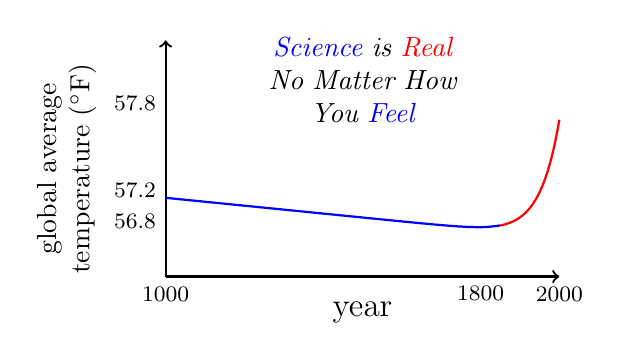
\begin{tikzpicture}
  \def \OX {0.}
  \def \OY {0.}
  \def \LX {5.}
  \def \LY {3.}
  \def \TY {2.5}
  \def \PI {3.14159}
  \draw [black,thick,->] (\OX,\OY) node[black,below] {\footnotesize 1000}
  -- (\LX,0) node[black,below] {\footnotesize 2000};
  \draw (4,0) node[black,below] {\footnotesize 1800};
  \draw (2.5,-0.2) node[black,below] {\large year};
  \draw [black,thick,->] (\OX,\OY) 
  -- (0,\LY) node[black,left,rotate=90,text depth=20ex,text width = 3cm,align=center] 
  {global average\\temperature (\degree F)};
  \draw (0,1.1) node[black,left] {\footnotesize 57.2};
  \draw (0,0.7) node[black,left] {\footnotesize 56.8};
  \draw (0,2.2) node[black,left] {\footnotesize 57.8};
 
  \draw [scale=1,domain=0:4.25,variable=\x,color=blue,thick,smooth]
  plot ({\x},{1 - 0.1*\x + exp(4*(\x-4.9))});
  \draw [scale=1,domain=4.25:5,variable=\x,color=red,thick,smooth]
  plot ({\x},{1 - 0.1*\x + exp(4*(\x-4.9))});

  \draw (\LX/2,\TY) node[align=center,text width=3cm] 
  {\it {\color{blue}Science} is {\color{red}Real}
    \\No Matter How\\You {\color{blue}Feel}};

\end{tikzpicture}
}
}
\end{picture}
\end{document}